%!TEX program = xelatex
\documentclass[11pt,punct,twoside]{ctexart}
\usepackage{titling}
\usepackage[a4paper, left=3cm, right=2cm, top=3cm, bottom=2.5cm]{geometry}
\usepackage{fancyhdr, graphicx, xpatch, layout}
\usepackage{booktabs}
\usepackage{amsmath}
\usepackage{pdfpages}
\usepackage{float}
%\usepackage{cite}
\usepackage{enumitem}
\usepackage{titlesec}
\usepackage{titletoc}
\usepackage[colorlinks,linkcolor=black,citecolor=black,urlcolor=black,bookmarks=false]{hyperref}
\usepackage{tabularx}
\usepackage{chngcntr}
\usepackage{listings}
\usepackage{cleveref}
\usepackage{subfigure}
\usepackage[titles,subfigure]{tocloft}
\usepackage[labelsep=space]{caption}
\usepackage[numbers,super,square,comma,sort,compress]{natbib}
\usepackage{lmodern}
\usepackage{indentfirst}
\usepackage{xtab,booktabs}
\usepackage[version=4]{mhchem}
\usepackage{array}
\usepackage{fontspec}
\usepackage{caption}
\usepackage{xeCJK}
\usepackage{color}
\usepackage{longtable}
%\usepackage{longtabu}
\usepackage{tabu}
\usepackage{makecell}
%\usepackage{showframe}

% 微分算子
\newcommand*{\dif}{\mathop{}\!\mathrm{d}}

% 参考文献行间距
\setlength{\bibsep}{-1pt}
%设置字体
\setmainfont{Times New Roman} % set all eng font
\songti%正文宋体
\zihao{-4}%正文小四号
\ctexset{section={format+={\mdseries\zihao{3}\heiti},aftername = \hspace{0.5em}}}%章标题 三号黑体
\ctexset{subsection={format+={\mdseries\zihao{-4}\heiti},aftername = \hspace{0.5em}}}%节标题 小四号黑体
\ctexset{subsubsection={format+={\mdseries\zihao{-4}\heiti},aftername = \hspace{0.5em}}}%级标题 小四号黑体  

%宋体伪粗体
\setCJKfamilyfont{zhsong}[AutoFakeBold = {2.17}]{SimSun}
\renewcommand*{\songti}{\CJKfamily{zhsong}}
%设置间距
\renewcommand{\baselinestretch}{1.62}
%\linespread{1.5}
\titlespacing{\section}{0bp}{0.5em}{0.5em}
\titlespacing{\subsection}{0bp}{0.5em}{0.5em}
\titlespacing{\subsubsection}{0bp}{0.5em}{0.5em}
%\setlength{\parskip}{0.5\baselineskip}
% 图表公式每章重新编号
\counterwithin{table}{section}
\counterwithin{figure}{section}
\counterwithin{equation}{section}

%表标题与内容间距
\setlength{\abovecaptionskip}{0.1cm}
%列表样式
\setlist[enumerate,1]{label=(\arabic*), wide, labelsep=0.5em, itemsep=0ex, topsep=0pt, partopsep=0pt, parsep=0pt}
\setlist[enumerate,2]{label=(\alph*) , wide, labelsep=0.5em, itemsep=0ex, topsep=0pt, partopsep=0pt, parsep=0pt,itemindent=5em}

%正文代码块lstlisting样式
\def\inline{\lstinline[basicstyle=\ttfamily,breaklines=true]}
\lstset{
	basicstyle=\ttfamily\zihao{5},
	xleftmargin=2em,
	%xrightmargin=2em,
    breaklines=true,
    frame={tb},
    belowcaptionskip=0.6em,
    framerule=1.5pt
}

%引用样式
\renewcommand{\lstlistingname}{代码清单}
\crefname{listing}{代码清单}{代码清单}
\crefname{table}{表}{表}
\Crefname{table}{表}{表}
\crefname{figure}{图}{图}
\Crefname{figure}{图}{图}

%自定义命令
\newcommand{\scite}[1]{\textsuperscript{\cite{#1}}} %cite样式
\DeclareCaptionFormat{myformat}{\zihao{5}\selectfont#1#2#3}
\captionsetup{format=myformat}
\captionsetup{labelsep=quad}%图表号与图表名之间空两格
\newcommand{\specialsection}[1]{% 正文后诸如“致谢”之类的章节,解决超链接问题
  \phantomsection
  \addcontentsline{toc}{section*}{\heiti\zihao{-4}#1}
  \section*{#1}
}

%------------------文档开始------------------
\begin{document}
\pagestyle{empty}
\begin{titlepage}
	\begin{figure}[t]
		\centering
		
\includegraphics[width=0.92\textwidth]{images/cover.png}
	\vspace{-2.5em}
	\end{figure}
	
	\begin{center}
		\quad \\
		\quad \\
		\heiti \zihao{-0} 毕业论文
		\vskip 0.5em
		\heiti \zihao{2} Mg/Al复合板材轧制过程微观组织和力学性能研究
	\end{center}
	\vskip 1em
	
	\makeatletter
	
	\newcommand\dlmu[2][8em]{\underline{\hb@xt@ #1{\hss#2\hss}}}
	\newcommand{\kernword}[1]{\expandafter\kernwordaux#1\relax}
	\def\kernwordaux#1{%
		\ifx\relax#1\else
		#1\hspace{0.05cm}\expandafter\kernwordaux % 这里调整下面表项的字距 默认0.05cm 实际自行调整
		\fi}
	\makeatother	
	\begin{center}
		\zihao{-3}
		\heiti
		\renewcommand\arraystretch{0.72} 
		\setlength\extrarowheight{5mm} 
		\begin{tabular}[b]{b{-0.5em}b{4em}b{0.25em}b{16em}<{\centering}}
			%\cline{4-4}
			&\makebox[4em][s]{院\ \ \ \ \ \ \ \ 别}  &   &\bf{\kernword{XXX学院}} \\
			\cline{4-4}
			&\makebox[4em][s]{专业名称}    &   &\bf{\kernword{XXX工程}} \\
			\cline{4-4}
			&\makebox[4em][s]{班级学号}    &   &\bf{\kernword{1601-20165678}} \\  % 加粗+字距
			\cline{4-4}
			&\makebox[4em][s]{学生姓名}    &   &\bf{\kernword{李XX}} \\ 
			\cline{4-4}
			&\makebox[4em][s]{指导教师}    &   &\bf{\kernword{XXX\ \ 教授}} \\
			\cline{4-4}
		\end{tabular}
	\end{center}

%多行注释
% \iffalse
% 	\begin{center}
% 		\zihao{-3}
% 		\heiti
% 		\renewcommand\arraystretch{1.08} 
% 		\setcellgapes [b]{0.5mm}
% 		\begin{tabular}[b]{rl}
% 			&\makebox[4em][s]{院\ \ \ \ \ \ \ \ 别}	\quad		\dlmu[16em]{X X X 学\ 院}      \\
% 			&\makebox[4em][s]{专业名称}	\quad	\dlmu[16em]{X X X 工\ 程}   \\
% 			&\makebox[4em][s]{班级学号}	\quad	\dlmu[16em]{\bf{1601-20165678}}   \\
% 			&\makebox[4em][s]{学生姓名}	\quad	\dlmu[16em]{李 X X}   \\ 
% 			&\makebox[4em][s]{指导教师}	\quad	\dlmu[16em]{X X X \ \ \ \ 教\ 授}   \\
% 		\end{tabular}
% 	\end{center}
% \fi


% 日期
\vskip 1em
\centering
\zihao{-3} \bf{202X}年\bf{X}月



\end{titlepage}
\cleardoublepage
\hspace*{\fill} \\
%\hspace*{\fill} \\

\section*{\textbf{\songti\zihao{2} 郑\ \ 重\ \ 声\ \ 明}}

%页眉页脚
\thispagestyle{fancy}
\lhead{}
\chead{\zihao{4}\heiti\ 东北大学秦皇岛分校本科生毕业设计(论文)} %\bfseries 不用加粗
\rhead{}
\fancyfoot{}


\hspace*{\fill} \\

{\zihao{4}\songti 本人呈交的学位论文,是在导师的指导下,独立进行研究工作所取得的成果,所有数据、图片资料真实可靠。尽我所知,除文中已经注明引用的内容外,本学位论文的研究成果不包含他人享有著作权的内容。对本论文所涉及的研究工作做出贡献的其他个人和集体,均已在文中以明确的方式标明。本学位论文的知识产权归属于培养单位。\par
 \hspace*{\fill} \\
 \hspace*{\fill} \\
 \hspace*{\fill} \\
 \hspace*{\fill} \par
本人签名: \makebox[3cm]{           }\ \ \ \  日期:
}
\cleardoublepage




%页眉页脚
\pagestyle{fancy}
%\setlength{\voffset}{3pt}
\lhead{}
\chead{\zihao{4}\heiti 东北大学秦皇岛分校本科生毕业设计(论文)} %\bfseries 不用加粗
%\textcolor{red/blue/green/black/white/cyan/magenta/yellow}{text}
\rhead{}
\lfoot{}
\cfoot{\zihao{5}\thepage}
\rfoot{}

\setlength{\voffset}{-10mm}                        
\setlength{\topmargin}{0mm}
\setlength{\headheight}{6mm}
\setlength{\headsep}{9mm}
\setlength{\footskip}{7.5mm}
\pagenumbering{Roman} %目录页码为罗马数字
\setcounter{page}{1}%页码重新计数

%正文代码块章节编号
\counterwithin{lstlisting}{section}

\section*{\zihao{-3}\heiti 基于XXXXXXX}
\section*{\zihao{3}\heiti 摘\ \ \ \  要}

写上你自己的摘要
\\
%空一行
\\
\zihao{-4}{\heiti 关键词:}啦啦啦;saki酱saki酱saki酱;随便;

\clearpage


\section*{\zihao{-3}\bfseries The Design of XXXX}

%\hfill Author: xxxx

%\hfill Tutor: xxxx

\section*{\zihao{3}\bfseries Abstract}

WRITE UR OWN ABSTRACT
	\\
	%空一行
	\\
	\zihao{-4}{\bfseries Key words:\ }Anything; WOW; Latex;

\clearpage





%目录样式
% \renewcommand{\cftdot}{\ensuremath{\ast}}
\titlecontents{section}
              [1em]
              {\heiti\zihao{-4}}%
              {\contentslabel{1em}}%
              {}%
              {\titlerule*[0.32pc]{$\cdot$}\contentspage}
\titlecontents{subsection}
              [3.5em]
              {\songti\zihao{-4}}%
              {\contentslabel{1.7em}}%
              {}%
              {\titlerule*[0.32pc]{$\cdot$}\contentspage}
\titlecontents{subsubsection}
              [6em]
              {\songti\zihao{-4}}%
              {\contentslabel{2.5em}}%
              {}%
              {\titlerule*[0.32pc]{$\cdot$}\contentspage}
\titlecontents{section*}
              [0em]
              {\heiti\zihao{-4}}%
              {\contentslabel{3em}}%
              {}%
              {\titlerule*[0.32pc]{$\cdot$}\contentspage}
\titlecontents{subsection*}
              [1em]
              {\songti\zihao{-4}}%
              {\contentslabel{1.7em}}%
              {}%
              {\titlerule*[0.32pc]{$\cdot$}\contentspage}
\renewcommand{\cftsecleader}{\cftdotfill{\cftdotsep}}
\newcommand\mydot[1]{\scalebox{#1}{.}}
\renewcommand\cftdot{\mydot{0.8}}
\renewcommand\cftdotsep{1}

%\captionsetup[contentsname={\zihao{3}目\ \ \ \ \ \ \ \ 录}]
\renewcommand{\contentsname}{\zihao{3}目\ \ \ \ \ \ \ \ 录}
\renewcommand{\cftsecfont}{\heiti\zihao{-4}} %设置section条目的字体
\renewcommand{\cftsecfont}{\heiti} %设置section条目的字体
%\renewcommand{\cftsecpagefont}{\normalfont}
\renewcommand{\cftsubsecfont}{\songti\zihao{-4}} %设置subsection条目的字体
\rhead{}
\tableofcontents
\cleardoublepage
\pagenumbering{arabic} %正文页码为阿拉伯数字
\section{绪论}
\subsection{引言}

镁及其合金是目前工业应用中密度最低的工程金属材料,密度在1.75~1.90g/cm³之间。镁合金比强度和比刚度高、具有优良电磁遮蔽性和的抗冲击性。并且易于加工,有良好的机械性能,制备简单、方便,可回收性高,因而被誉为“21世纪绿色结构材料”\cite{a1,i2}。镁合金被用作各种优质工业合金的基础材料,在于航空航天、国防、电子、交通运输、尤其是汽车工业等领域有着广泛的应用前景\cite{a1,a3,i4}。\par

\subsection{研究背景}
\subsubsection{国外研究现状}

镁是一种比铝还轻的轻金属,密度约为1.74g/cm³,熔点约为650℃。镁的晶体结构为密排六方,是地壳中存储较多的金属之一,达到2.1$\%$,占据第三位,仅次于Al和Fe。镁广泛存在于地壳中,同时大量储存于海水中。\par

\subsubsection{国内研究现状}

按工艺来分,镁合金有变形镁合金和铸造镁合金两大类,一般来说,通过锻造、轧制、挤压等方法制备的镁合金被称为变形镁合金,产品往往用于汽车行业、航空航天及军工行业。铸造镁合金的特点是可在相同的强度条件下减轻工件质量,可代替铝合金铸件在汽车零件和电器构件中的应用。变形镁合金在变形加工过程中通过成型工艺的选择和控制、结合热处理工艺,可使其显微组织细化,消除缺陷,可获得更高的强度、更好的延展性和更多样化的力学性能,从而满足更复杂多变工程结构件的应用需求,所以在实际生产中对变形镁合金的需求更大,对变形镁合金的研究也是当下研究热点。\par

\subsection{层状复合轧制工艺研究现状}
\subsubsection{复合轧制工艺概述}

复合轧制是将两层或多层金属或合金叠放在一起进行轧制,依靠原子之间金属键的相互吸引力而使金属复合的一种工艺。复合轧制可使两种或多种物理、化学和力学性能不同的材料在界面上实现牢固的冶金结合。目前以发展了多种复合工艺,包括热轧复合、冷轧复合、爆炸复合、异步轧制复合和堆焊等方法。\par
\subsection{铝/镁层状金属复合轧制研究现状}

目前国内外对铝/镁复合轧制工艺的研究还未取得较大进展,研究表明,利用累积叠轧(Accumulative roll bonding)可以较好的实现镁、铝金属的复合。ARB属于金属材料的严重塑性变形(SPD)(正文中括号全角状态下的括号)工艺的一种,在循环中包括,多次轧制、切割、堆垛和固态变形粘合。使金属发生严重的塑性变形,产生大块超细的晶界结构。铝/镁层状金属利用累积叠轧技术制备,可有效提升复合板材的晶界结构,提高硬度等综合性能。它能够实现低成本效益高的连续制造,所以该技术具有很好的商业化潜力。\par
\subsection{本文的研究意义和主要内容}

因为镁合金具备许多优点,在诸多领域有着广泛的应用,然而应用的范围却被腐蚀性差等缺点限制。另一方面,纯铝具有良好的耐腐蚀性。通过轧制方法制成Al/Mg/Al复合板材,实现外层铝对中心层镁层的包覆。让复合材料兼具镁合金的高比强度和铝合金优良的耐腐蚀性能。同时,镁、铝的结合还能提升材料的整体塑性和变形抗力,延缓镁合金变形过程中裂纹的扩展。这种复合材料在航天航空以及汽车领域具有巨大的潜力。本文对于提升镁铝复合板材的生产水平、突破镁合金的应用局限有一定的现实意义。\par

\clearpage
\section{实验材料及方法}
本文是将商用AZ31B镁合金板材和1060纯铝板材制成铝-镁-铝夹层,进行不同道次及道次压下率复合轧制实验,并对轧制所得板材进行显微组织观察及力学性能分析研究。本章介绍了实验所采用的材料、样品制备方式及实验方法。\par
\subsection{实验流程图}
图\ref{fig:liuchengtu}所示为实验流程图。对试样轧制复合后,主要利用相关仪器设备测试分析微观组织和力学性能。\par

%顶部对齐,将空白集中到页面底部
\raggedbottom

\begin{figure}[H]
	\vspace{-0.5em}
	\centering
	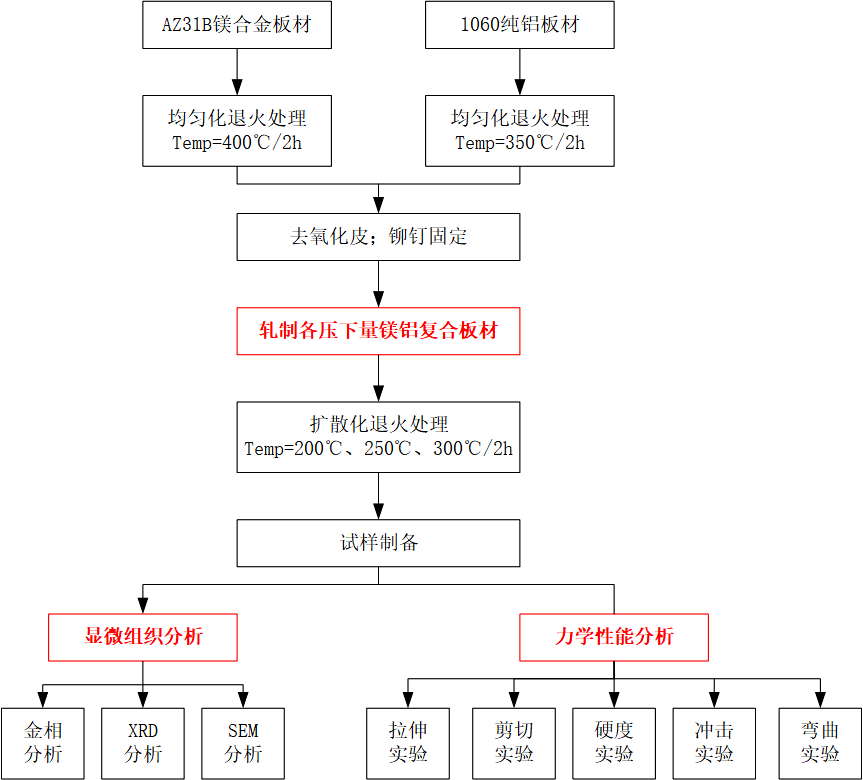
\includegraphics[width=0.8\textwidth]{images/liuchengtu.png}
	\caption{情感倾向分析流程}
	\label{fig:liuchengtu}
	\vspace{-1.5em}
\end{figure}
\subsection{实验材料}
实验所采用的原始材料为商用AZ31B镁合金铸轧板材和1060铝板材。合金原材料采用连续铸轧工艺生产,生产工序经过配料/熔炼/静置/放料/连续铸轧等流程,由于原材料板材较大,采用剪板机进行切割取样。\par
\subsection{样品制备}
\subsubsection{镁铝夹层的制备}
轧制前准备好8块镁合金板材和16块铝合金板材样品,镁板和铝板厚度均为2mm,将镁板放入加热炉进行400℃均匀化退火处理2小时,铝板放入加热炉进行350℃均匀化退火处理2小时。\par


\subsubsection{金相试样制备}
因为轧制获得的镁铝复合板材存在边缘裂纹等缺陷,需要利用线切割机床进行切割取样,其中金相观察部分中,对未退火及各退火温度(200℃、250℃、300℃)的轧制后板材各取3个试样,切割成矩形小块,分别用于观察表面金相组织、镁铝界面相组织。\par
\subsubsection{XRD试样制备}
制备XRD试样时,先用600$\#$、1000$\#$、2000$\#$砂纸将表面打磨平整、去除表面氧化皮并清洁干净,随后取一张干净的滤纸,将样品放置在铝合金框架中间,用橡皮泥固定,使待观察的试样表面与铝合金框架平齐,处于同一平面上。\par
\subsection{实验方法}
\subsubsection{金相观察}
在金相观察前,先用普通光学显微镜观察腐蚀效果,如能观察到清晰的晶界且没有明显缺陷,则改用金相显微镜观察记录,观察时进行图像采集并添加标尺。\par
\subsubsection{扫描电镜(SEM)分析}
扫描电镜(SEM)的主要原理是利用聚焦电子束照射在试样表面所激发出来的一系列物理信号所形成的图像。入射电子束和样品表面作用后会产生很大电子信号,譬如吸收电子、背散射电子、透射电子、二次电子和特征 X 射线。 \par

\clearpage
\section{Al/Mg/Al复合板材微观组织分析}

	为探究不同轧制条件下镁铝复合板材的性能变化,本章通过分析金相组织、扫描电镜分析、XRD衍射分析、拉伸实验、弯曲实验、冲击实验和剪切实验及表面维氏硬度测试的实验结果,探究镁铝复合板材的组织、性能变化的特点并探究其原因。\par
	
	\subsection{金相组织分析}		  
		\subsubsection{压下量变化对金相组织的影响}
		\begin{enumerate}
			\item 镁层ND-RD面金相组织变化
			
			不同压下量下复合板材中间镁层金相显微组织如图3.1所示。其中辊面温度为300℃,轧制速度为0.03 m/s,RD为轧制方向,ND为厚度方向。
			
			\item 结合面金相组织变化
			
			如图3.2所示为辊面温度为300℃,不同压下率下轧后Al/Mg/Al复合板镁层与铝层结合面金相组织。
		\end{enumerate}
		\subsubsection{退火温度对金相组织的影响}
		在本次实验中,经过轧制后的镁铝复合板材,因为镁合金的滑移系较少,在轧制过程中不易发生宏观屈服,因此会在晶界处造成应力集中,Al/Mg/Al层合板中的外层铝层所承受的较大变形是由板与辊之间的摩擦引起的相对较大的剪切应变引起的,导致了铝层很强的加工硬化。此时镁铝复合板的内能、强度硬度都比较高,处于亚稳态状态。\par

		\subsubsection{晶粒大小与平均尺寸分布图}
		对比原始板材的晶粒大小分布可发现,原始板材本身的晶粒尺寸分布很不均匀,在各个轧制压下率下,而在压下率提升后,均匀性有了很大程度的改善,其中,73$\%$和83$\%$压下量板材镁层晶粒尺寸最细小,83$\%$压下量板材镁层晶粒均匀性最高。分布的均匀性也影响到了复合板材的力学性能。\par
	\subsection{扫描分析}			
		\subsubsection{Al/Mg/Al复合板材微观形貌}
		本实验中镁层和铝层之间的结合良好,界面之间没有裂缝、空洞或界限。从图中可以看到随着变形率的提高,镁层的厚度逐渐降低,两种组分金属在各个变形量轧制下的变形基本均匀并保持了良好的连续性,增大压下率,当变形量达到73$\%$,可以观察到波纹结构。\par
		\subsubsection{Al/Mg/Al复合板材剥离面微观形貌}
		\begin{enumerate}
			\item 镁层剥离面微观形貌
			
			通过扫描数据可知,镁层上生成的中间相的原子镁元素的质量百分比为50.74$\%$,铝元素的质量百分比为46.69$\%$,原子比接近17:12。
			
			\item 铝层剥离面微观形貌
			
			扫描数据显示,镁层上生成的中间相的原子镁元素的质量百分比为44.97$\%$,铝元素的质量百分比为53.18$\%$,原子比接近2:3。
		\end{enumerate}
	\subsection{XRD分析}	
		为了进一步确认中间结合层物相的成分并探究不同退火条件对中间层含量的影响,对各组样品进行了XRD实验,利用JADE软件对实验数据进行分析。\par
		对数据进行分析和拟合得到元素扩散模型见公式\eqref{e1}和\eqref{e2}:\par
	\vspace{-2em}
	\begin{equation} \label{e1}
		\begin{split}
			&f(x,y)=[f(1,0)-f(0,0)]x+[f(0,1)-f(0,0)]y \\
			&+[f(1,1)+f(0,0)-f(0,1)]xy+f(0,0) 
		\end{split}
	\end{equation}
	\vspace{-1em}
	\begin{equation} \label{e2}
		\begin{split}
			f(x,y)&=[f(1,0)-f(0,0)]x+[f(0,1)-f(0,0)]y \\
			&=[f(1,1)+f(0,0)-f(0,1)]xy+f(0,0) 
		\end{split}
	\end{equation}	
		
 \clearpage


\specialsection{结\ \ \ \ \ \ \ \ 论}
% \section*{结\ \ \ \ \ \ \ \ 论}
% \addcontentsline{toc}{section*}{结\ \ \ \ \ \ \ \ 论}


	本文针对AZ31B镁合金板材和1060纯铝板材在辊面温度300℃条件下进行复合轧制,成功制备出了Al/Mg/Al层状复合板材。研究了在不同轧制压下率条件和不同退火温度条件下的显微组织性能与力学性能变化,主要结论如下:\par
	\begin{enumerate}
		\item 随着轧制变形量的增加,复合板材镁层、铝层厚度不断降低、第一道次下降幅度较大,随后变化幅度较低,这是由于加工硬化导致变形能力减弱。中心镁层组织随着塑性变形的累积,由原始母材的粗大等轴晶先被拉长成为细长晶粒后变成细小的等轴晶。
		
		\item 通过XRD衍射图谱和SEM线扫描图谱分析,当压下率较低时轧后板材未发现金属间化合物,但在后续扩散退火中析出第二相,而压下率为73$\%$和83$\%$时轧制候复合板材出现金属间化合物Mg17Al12和Al3Mg2。由于加工硬化机制和细晶强化机制共同作用,复合板材的综合力学性能得到提升。
		
		\item 退火处理可以消除残余应力和减少内部缺陷,退火温度升高促进了异种材料界面处镁铝原子相互扩散。 
				
	\end{enumerate}
	
\specialsection{致\ \ \ \ \ \ \ \ 谢}
% \section*{致\ \ \ \ \ \ \ \ 谢}
% \addcontentsline{toc}{section*}{致\ \ \ \ \ \ \ \ 谢}

	致谢致谢致谢致谢致谢致谢致谢致谢致谢致谢致谢致谢致谢致谢致谢致谢致谢致谢致谢致谢致谢致谢致谢致谢致谢致谢致谢致谢致谢致谢致谢致谢致谢致谢致谢致谢致谢致谢致谢致谢致谢致谢。\par
	

\bibliographystyle{gbt7714-2005}
%\bibliographystyle{unsrt}
\nocite{*}
\phantomsection
\addcontentsline{toc}{section*}{参考文献}

\renewcommand\bibnumfmt[1]{\makebox[0.9cm][l]{[#1]}}
\setlength{\bibhang}{0em}

\bibliography{citation}

\appendix

\specialsection{附\ \ \ \ \ \ \ \ 录}
% \section*{附\ \ \ \ \ \ \ \ 录}

% \addcontentsline{toc}{section*}{附\ \ \ \ \ \ \ \ 录}

%创建单独appendix计数器,解决目录中附录样式问题

\newcounter{appendix}
\setcounter{appendix}{1}

% \renewcommand{\thesubsection}{附录\Alph{subsection}}

\newcommand{\appendsection}[1]{
	\titleformat*{\subsection}{}
	\zihao{-4}\heiti
	\phantomsection
	\addcontentsline{toc}{subsection*}{附录\Alph{appendix}}
	\subsection*{附录\Alph{appendix}}
	{\centering\paragraph{#1}\mbox{}\\}\songti
}


% 单独使用\appendsection时,请自行在下面添加\stepcounter{appendix},否则编号将异常
\newcommand{\appendchn}[1]{
	\titleformat*{\subsection}{}
	\zihao{-4}\heiti
	\subsection*{中文译文\Alph{appendix}}
	\stepcounter{appendix} %在此处appendix计数器加1,意味着单独附录章节结束
	{\centering\paragraph{#1}\mbox{}\\}\songti
}


\appendsection{Analysis on Risk Prevention of Tax Planning in Real Estate Development Enterprise}
	Tax planning refers that taxpayer deals with financial, operating, organizing and other business proceedings in range of tax law so as to delay or alleviate enterprise taxes and realize the largest benefit after paying taxes.\par
	
\appendchn{分析纳税筹划在房地产开发企业的风险防范}
	税收筹划是指纳税人在税法的范围内处理财务,经营,组织其他商业活动的过程,以拖延或减轻企业的税收和实现纳税后的最大的效益。\par
\clearpage

\appendsection{Analysis on Risk Prevention of Tax Planning in Real Estate Development Enterprise}
Tax planning refers that taxpayer deals with financial, operating, organizing and other business proceedings in range of tax law so as to delay or alleviate enterprise taxes and realize the largest benefit after paying taxes.\par

\appendchn{分析纳税筹划在房地产开发企业的风险防范}
税收筹划是指纳税人在税法的范围内处理财务,经营,组织其他商业活动的过程,以拖延或减轻企业的税收和实现纳税后的最大的效益。\par
\clearpage

% 代码段未测试 按需使用 应该没问题

\appendsection{代\ \ \ \ \ \ \ \ 码}
%取消章节编号,重置计数器
\counterwithout{lstlisting}{section}
\setcounter{lstlisting}{0}
%附录代码风格
\lstset{
	basicstyle          =   \sffamily,          % 基本代码风格
	keywordstyle        =   \bfseries,          % 关键字风格
	commentstyle        =   \rmfamily\itshape,  % 注释的风格,斜体
	stringstyle         =   \ttfamily,  % 字符串风格
	flexiblecolumns,                % 别问为什么,加上这个
	numbers             =   left,   % 行号的位置在左边
	showspaces          =   false,  % 是否显示空格,显示了有点乱,所以不现实了
	numberstyle         =   \zihao{-5}\ttfamily,    % 行号的样式,小五号,tt等宽字体
	showstringspaces    =   false,
	captionpos          =   t,      % 这段代码的名字所呈现的位置,t指的是top上面
	frame               =   lrtb,   % 显示边框
	framerule           =   0.5pt,  % 边框宽度
}

\lstdefinestyle{Python}{
	language        =   Python, % 语言选Python
	basicstyle      =   \zihao{-5}\ttfamily,
	numberstyle     =   \zihao{-5}\ttfamily,
	keywordstyle    =   \color{blue},
	keywordstyle    =   [2] \color{teal},
	stringstyle     =   \color{magenta},
	commentstyle    =   \color{red}\ttfamily,
	breaklines      =   true,   % 自动换行,建议不要写太长的行
	columns         =   fixed,  % 如果不加这一句,字间距就不固定,很丑,必须加
	basewidth       =   0.5em,
}
\subsubsection*{1.情感分析}
\lstinputlisting[
style       =   Python,
caption     =   {qg.py},
label       =   {qg.py}
]{images/qg.py}


\end{document}